\documentclass[11pt]{article}
\usepackage[margin=1in]{geometry}
\usepackage{volfit_preamble}
\graphicspath{{figures/}}

\title{\textbf{The Unnamed Martingale}\\[2pt]
\large Calendar order as an existence theorem, and who pays to
restore it\\[2pt]
\normalsize Vol-Fitter Technical Notes, No.~10}
\author{Vol-Fitter}
\date{\today}

% Note-local notation (shared symbols come from volfit_preamble).
\newcommand{\cx}{\le_{\mathrm{cx}}}
\newcommand{\Lo}{\Lambda}

\begin{document}
\maketitle

% Generated numbers.  cal_martingale_tables.tex carries everything unique
% to this edition (gen_cal_martingale.py).  Never retype a generated number.
% Auto-generated by gen_cal_martingale.py — do not edit.
\newcommand{\calmheronodes}{6}
\newcommand{\calmheromarginbp}{0.9}
\newcommand{\calmherophantombp}{21}
\newcommand{\calmfacesminspread}{\ensuremath{4.8\times10^{-4}}}
\newcommand{\calmdragfreebp}{10.6}
\newcommand{\calmdragfullbp}{1095}
\newcommand{\calmdragwinbp}{228}
\newcommand{\calmdragpricebp}{10.6}
\newcommand{\calmviolfree}{0.0058}
\newcommand{\calmviolcured}{\ensuremath{3.2\times10^{-6}}}
\newcommand{\calmseqnearbp}{4.8}
\newcommand{\calmseqfarbp}{547}
\newcommand{\calmsymnearbp}{414}
\newcommand{\calmsymfarbp}{254}
\newcommand{\calmphantomwidebp}{151}
\newcommand{\calmphantomdatabp}{0.0}
\newcommand{\calmrefagree}{\ensuremath{1.0\times10^{-17}}}
\newcommand{\calmgencommit}{7933d17}
\newcommand{\calmgendate}{2026-07-19}


\begin{abstract}
A fitted surface makes a promise it never spells out: that \emph{some}
arbitrage-free dynamics --- a martingale the fitter neither builds nor
names --- could produce exactly these smiles.  This lecture develops
calendar-arbitrage prevention from that existence statement.  By
Kellerer's theorem the promise is precisely checkable: butterfly-free
slices increasing in convex order admit a martingale with those
marginals, and convex order has four equivalent inspection coordinates
--- normalized calls, the laws themselves, integrated upper-quantile
curves, total implied variance --- so each model verifies the one it
already owns (for LQD the integrated-quantile curve \emph{is} the
asset-share array every built slice carries; the parametric overlays
hinge total variance against the previous displayed slice; the local-vol
surface keeps the promise by construction).  On a live SPY surface the
promise holds with a margin of \calmheromarginbp\ variance bp everywhere
two expiries are jointly quoted, while their drawn extrapolations
disagree by up to \calmherophantombp\ variance bp --- which is why
\emph{where} the order is inspected is half the design: the confinement
case file (the phantom calendar that flattened live NVDA and SPY fits,
reproduced here at \calmphantomwidebp\ vol bp of damage under a wide
floor grid vs \calmphantomdatabp\ under the confined one) and a measured
rejection of the quantile coordinate for confinement --- a $G$-space
floor drags an innocent far fit by \calmdragfullbp\ vol bp, still
\calmdragwinbp\ after windowing, because $G$ integrates the whole upper
tail; the production floor compares \emph{prices at fixed strike},
\calmdragpricebp\ bp, indistinguishable from no floor.  The other half
is \emph{who pays} when slices genuinely conflict: the historical
sequential pass bulldozes the latecomer (near untouched at
\calmseqnearbp\ bp, far conceding \calmseqfarbp), while the shipped
symmetric solver --- independent fits, a vega-normalized screen, then
one joint Gauss--Newton over the violating component --- shares the
concession (\calmsymnearbp/\calmsymfarbp\ bp), cures the order to
\calmviolcured\ in total variance, and leaves clean ladders
byte-identical to their independent fits.
\end{abstract}

\newpage
\tableofcontents
\newpage

%======================================================================
\section{The promise}
\label{sec:promise}

\Cref{fig:hero} is a live SPY surface: six expiries, each fitted
independently well, drawn as one family.  Where two adjacent expiries
are both quoted, the later curve sits strictly above the earlier one ---
with a worst margin of \calmheromarginbp\ variance bp --- and that
ordering is not an aesthetic: it is the entire difference between six
good smiles and one coherent \emph{surface}.  A desk that trades the
surface trades between expiries: forward-starting variance, calendar
spreads, rolls.  Each such trade prices a claim on what happens
\emph{between} two slices, and the slices only admit a consistent
in-between if they stand in the right order.

\begin{figure}[H]
\centering
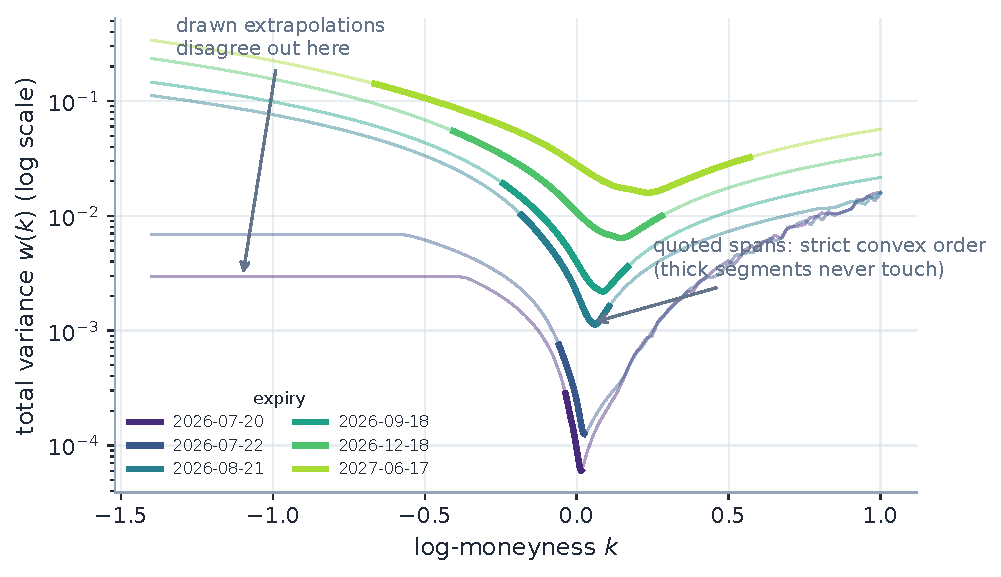
\includegraphics[width=0.92\textwidth]{fig_calm_hero.pdf}
\caption{The promise, held live (SPY, Massive feed, \calmheronodes\
expiries, published production fits).  Thick segments mark each slice's
quoted span: on every common traded span the later expiry dominates ---
convex order with \calmheromarginbp\ variance bp to spare at the
tightest pair.  The faint tails are the drawn extrapolations, which
disagree by up to \calmherophantombp\ variance bp out where no quote
exists --- the region \cref{sec:where} rules out of bounds for any
two-curve comparison.}
\label{fig:hero}
\end{figure}

This lecture is about what exactly that order buys, per model and per
pair of slices; the organizing statement is an \emph{existence
theorem}.  A butterfly-free slice (Notes~01--04) certifies that a valid
law exists at one date.  The calendar condition certifies something
stronger and strictly cross-sectional: that some \emph{martingale} ---
some arbitrage-free dynamics the fitter never constructs --- has
exactly these laws as marginals.  The fitter's product is a family of
still photographs; the promise is that a film exists whose frames they
are.  No frame is ever named, no film is ever shot, and yet the promise
is falsifiable frame by frame --- that is the content of
\cref{thm:faces} and \cref{thm:kellerer} below.

\begin{assumption}[Units and carry]
\label{ass:units}
Each expiry is normalized by its own forward: $Y_T=S_T/F_T$ (so
$\E[Y_T]=1$ for every $T$), quotes live at fixed log-moneyness
$k=\log(K/F_T)$, and rates, borrow and dividends are deterministic and
absorbed into $F_T$ (Note~06).  Comparisons across maturity are made at
fixed $k$ --- fixed \emph{forward} moneyness, not fixed cash strike.
Discrete cash dividends make the cash-strike statement fail while the
normalized one survives; stochastic rates would break the equivalence
between calendar spreads and the normalized comparison altogether.  The
event clock of Note~11 reparametrizes maturity within each slice but
preserves the \emph{ordering} of expiries (the dilated clock is
monotone), so nothing below is affected; the production expiry chain is
keyed by settlement instant, not calendar date.
\end{assumption}

\begin{invariant}
\begin{enumerate}[leftmargin=1.6em]
\item Where data lives, the fitted surface is increasing in convex
order: no calendar spread against it.
\item Enforcement is \emph{soft} --- quotes still win a genuine
conflict, and the diagnostics report what slack was used.
\item Calendar coupling off, or a clean ladder, is byte-identical to
independent fits (under the symmetric solver this is a verified fast
path, not an aspiration).
\item The order is inspected only where \emph{both} slices are pinned
by data, and inspected in \emph{price} space at fixed strike --- the
confinement principle (Note~09), sharpened here by a measured rejection
of the quantile coordinate (\cref{sec:where}).
\end{enumerate}
\end{invariant}

\paragraph{Conventions and the notation ledger.}
$T_1<T_2$ (or $i,j$) index expiries; $t$ is not used.  Subscripted
$\partial$ for derivatives; no primes.  A variance bp is $10^{-4}$ of
total variance; a vol bp is $10^{-4}$ of absolute volatility.

\begin{table}[H]
\centering\footnotesize
\setlength{\tabcolsep}{3pt}
\begin{tabular}{@{}llll@{}}
\toprule
$Y_T=S_T/F_T,\ k$ & normalized terminal; log-moneyness &
$C_T(k)=\E[(Y_T-e^{k})^{+}]$ & normalized call\\[2pt]
$\cx$ & increasing convex order &
$G_T(\alpha)=\int_\alpha^1 Q_T(u)\,\dd u$ & integrated upper quantile\\[2pt]
$Q_T,\ \Lo,\ z,\ \alpha$ & quantile fn; logistic; logit; level &
$\tvar_T(k)$ & total implied variance\\[2pt]
$A(z)$ & LQD asset share ($=G$, \cref{prop:GisA}) &
$W_{\mathrm{cal}}$ & hinge weight\\
\bottomrule
\end{tabular}
\caption{Every symbol in the note.  $G$ is always the integrated
quantile curve (Durrleman's $g$ never appears here); $\alpha$ is always
a quantile level.}
\label{tab:ledger}
\end{table}

%======================================================================
\section{The existence theorem}
\label{sec:exist}

\begin{theorem}[Four faces of calendar order]
\label{thm:faces}
Let $\{Y_T\}$ have unit mean, and for $T_1<T_2$ consider:
\begin{equation}
\boxed{\;
\begin{aligned}
C_{T_1}(k)\le C_{T_2}(k)\ \forall k
\;&\Longleftrightarrow\;
Y_{T_1}\cx Y_{T_2}\\[1pt]
\Longleftrightarrow\;
G_{T_1}(\alpha)\le G_{T_2}(\alpha)\ \forall\alpha
\;&\Longleftrightarrow\;
\tvar_{T_1}(k)\le \tvar_{T_2}(k)\ \forall k .
\end{aligned}
\;}
\label{eq:faces}
\end{equation}
All four are equivalent, with $G_{T_1}(0)=G_{T_2}(0)=1$ pinning the
means.
\end{theorem}

\begin{proof}[Proof sketch]
(i)$\Leftrightarrow$(ii): call payoffs $(y-e^{k})^{+}$ span the convex
functions of $y$ --- every convex $\phi$ with matching means integrates
against $\partial_{KK}$ of the call in strike, the
Breeden--Litzenberger pairing --- so ordering all calls at equal means
is exactly convex order \cite{Strassen1965,CarrMadan2005}; Exercise~1
walks the spanning direction.
(ii)$\Leftrightarrow$(iii): the Hardy--Littlewood characterization ---
$\E\phi(Y_1)\le\E\phi(Y_2)$ for all convex $\phi$ iff the integrated
quantile curves are ordered; $G$ is the upper-tail version.
(i)$\Leftrightarrow$(iv): the normalized Black price is strictly
increasing in total variance at fixed $k$, so ordering prices at every
$k$ is ordering the implied $\tvar$ at every $k$
\cite{GatheralJacquier2014}.
\end{proof}

\begin{theorem}[Kellerer: the promise made precise]
\label{thm:kellerer}
If each slice is butterfly-free (a valid density) and the family is
increasing in convex order --- a \emph{peacock}
\cite{HPRY2011} --- then there exists a martingale $\{M_T\}$ with
$\mathrm{law}(M_T)=\mathrm{law}(Y_T)$ for every $T$
\cite{Kellerer1972}.
\end{theorem}

This is why the note's title is not a metaphor.  Butterfly-freedom per
slice plus calendar order across slices is not merely ``no static
arbitrage'': it is exactly the statement that the surface is consistent
with \emph{some} arbitrage-free dynamic model.  The fitter checks a
static, per-pair, per-strike inequality; the theorem converts the check
into an existential guarantee about dynamics.  Everything the rest of
the note does --- choosing the inspection coordinate, confining the
inspection region, deciding who concedes when slices conflict --- is
engineering in service of \eqref{eq:faces}; the mathematics is settled
by the two theorems above.

\begin{heuristic}
Convex order with equal means says the longer law is a
\emph{mean-preserving spread} of the shorter: same forward, more
dispersion --- exactly what a diffusion does as variance accumulates.
Enforcing it between independently fitted expiries is what stops two
individually good slice fits from implying a negative forward variance
between them: at the money, face (iv) reads
$\tvar_{T_2}(0)-\tvar_{T_1}(0)\ge0$, and that difference \emph{is} the
forward variance a calendar position buys (Exercise~2).
\end{heuristic}

\Cref{fig:faces} draws all four faces for one ordered production pair.
The four panels are one fact in four coordinate systems, and the reason
to keep all four alive is practical: each model of this series happens
to hold exactly one of them at zero cost.

\begin{figure}[H]
\centering
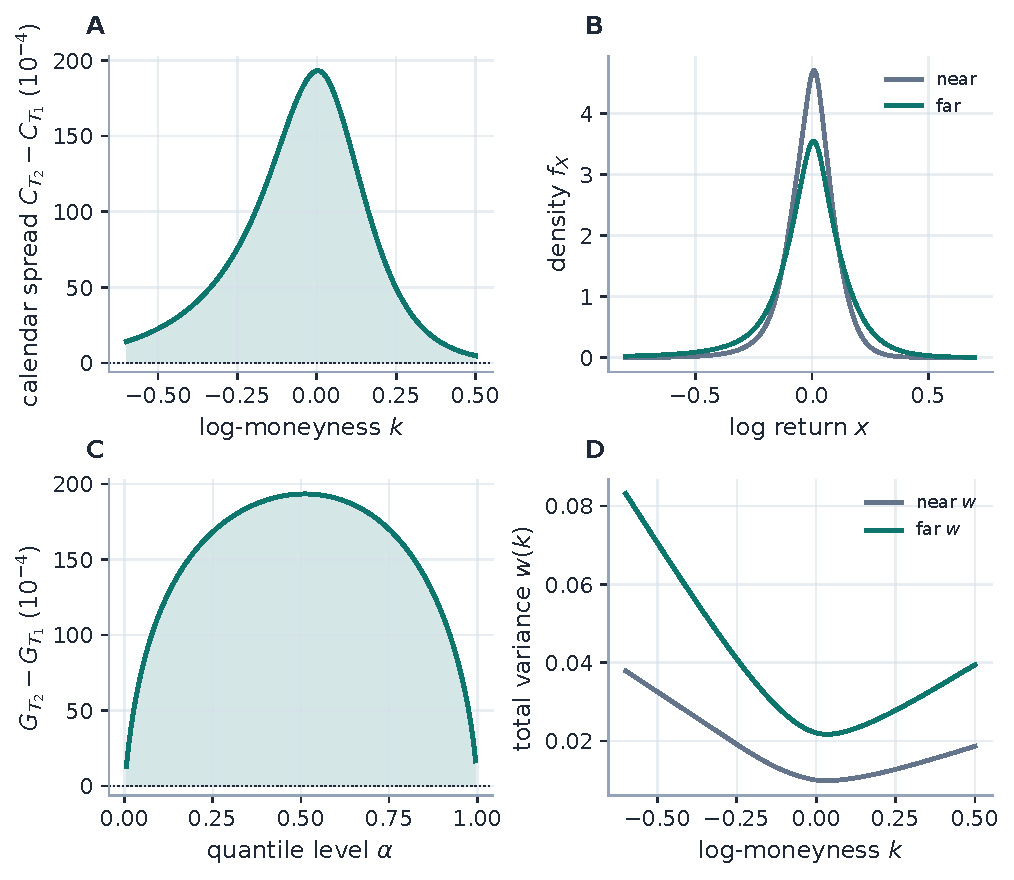
\includegraphics[width=0.94\textwidth]{fig_calm_faces.pdf}
\caption{One ordered pair, inspected in all four coordinates of
\eqref{eq:faces} (production LQD fits).  A: the calendar spread
$C_{T_2}-C_{T_1}$ is non-negative at every strike (min
\calmfacesminspread) --- face (i).  B: the far density is a
mean-preserving spread of the near one --- face (ii).  C: the
integrated-quantile gap $G_{T_2}-G_{T_1}$ is a non-negative dome,
pinched to zero at both ends by the equal means --- face (iii).  D:
total variance dominates pointwise --- face (iv).  Four inspections,
one order.}
\label{fig:faces}
\end{figure}

\paragraph{Exercise 1.}
Prove the spanning direction of (i)$\Rightarrow$(ii) for twice
continuously differentiable $\phi$: write
\[
\phi(y)=\phi(1)+\partial_y\phi(1)(y-1)
+\int_0^{1}\partial_{KK}\phi(K)(K-y)^{+}\dd K
+\int_1^{\infty}\partial_{KK}\phi(K)(y-K)^{+}\dd K
\]
(the same decomposition as Note~08's spanning proposition), take
expectations under both laws, and use equal means plus put--call parity
to reduce every term to ordered calls.

\paragraph{Exercise 2.}
The worked pair of \cref{sec:who} has ATM total variances
$\tvar_{T_1}(0)>\tvar_{T_2}(0)$ before repair (an event-inverted term
structure).  Compute the implied forward variance
$\big(\tvar_{T_2}(0)-\tvar_{T_1}(0)\big)/(T_2-T_1)$ from the free fits
of \cref{fig:solver}B and confirm it is negative --- the forward
volatility is imaginary, and a calendar position bought at these marks
locks in variance at a negative price.
The violation number \calmviolfree\ (in total variance) is the same
statement made uniform across strikes.

%======================================================================
\section{Four faces, one cheap check per model}
\label{sec:cheap}

The equivalence \eqref{eq:faces} would be idle if every check cost a
grid of Black inversions.  The design observation --- the same one
Note~08 made for the var-swap --- is that each model already owns one
face.

\subsection{LQD: the curve is already on the grid}

\begin{proposition}[The asset share is the integrated quantile curve]
\label{prop:GisA}
For an LQD slice with quantile $Q(z)$ in the logit coordinate
(Note~01),
\[
G(\alpha)=\int_\alpha^1 e^{Q(u)}\,\dd u
=\int_{z_\alpha}^{\infty}e^{Q(z)}\,\Lo(z)\big(1-\Lo(z)\big)\,\dd z
=A(z_\alpha).
\]
\end{proposition}

\begin{proof}
Substitute $u=\Lo(z)$, $\dd u=\Lo(1-\Lo)\,\dd z$ and compare with
Note~01's asset-share integral --- the same object.
\end{proof}

So face (iii) needs no new computation: every built slice carries
$A(z)$ on the shared quadrature grid, and the full-surface calendar
diagnostic is an elementwise comparison of two arrays, with constraint
points automatically dense in the wings (the grid is uniform in $z$,
not $k$).  As a \emph{fit-time} constraint the same face enters as a
soft squared hinge on a strided subgrid ($\sim$320 of the $8001$
nodes),
\begin{equation}
\sqrt{W_{\mathrm{cal}}}\,
\max\!\big(A_{T_1}(z_m)-A_{T_2}(z_m),\,0\big),
\qquad W_{\mathrm{cal}}=10^{6},
\label{eq:slack}
\end{equation}
keyed on the constraint $z$-\emph{coordinates}, so a slice calibrated
on a coarser optimization grid enforces it by Hermite evaluation,
bit-for-bit equivalent to the node-indexed form on the native grid.
Where this face is \emph{confined} rather than taken on the full grid,
production deliberately abandons it for face (i) --- \cref{sec:where}
measures why.

\subsection{SVI and MCS: face (iv) against the displayed neighbour}

The parametric overlays carry no quantile curve, so they hinge total
variance directly,
\begin{equation}
\sqrt{W_{\mathrm{cal}}}\,
\max\!\big(\tvar_{\mathrm{near}}(k_m)-\tvar_{\mathrm{far}}(k_m),\,0\big),
\label{eq:wfloor}
\end{equation}
on a data-confined log-moneyness grid, reading only the previous
\emph{displayed} slice's implied variance --- whatever model drew it
(and symmetrically against the next slice as a ceiling, so an overlay
refit cannot break the pair from above).  The production plumbing is
the part that took care: the floor needs the previous displayed slice,
so the calendar toggle threads it in ascending maturity through
\emph{every} path that fits a slice --- the single-slice overlay, the
commit path, the full-surface loop and the coupled workflow.  Wherever
the floor is absent (toggle off, or the first expiry) the residual
block is absent too: byte-identical, test-locked per model and per
path.

\subsection{Local volatility: the promise by construction}

The LV surface needs neither hinge.  A positive local variance makes
the Dupire march's continuum prices increasing in maturity at fixed
strike --- face (iv) holds along the whole solve --- so
calendar-cleanliness is structural (Note~04); production carries only a
discrete diagnostic (worst adjacent-expiry price decrease, tolerance
$10^{-8}$) to confirm the scheme respects what the continuum promises.
This mirrors Note~09's wing taxonomy: LQD structural in one dimension
is LV structural in the other --- a model built \emph{from} a valid
generator inherits the promise its coordinates encode.

%======================================================================
\section{Where the order may be inspected}
\label{sec:where}

Both hinges above compare \emph{two} curves, and Note~09's confinement
principle applies with full force: a two-curve constraint may be
sampled only where data pins both.  This section is the calendar's own
case file --- the incident that founded the principle --- plus this
edition's sharpening: confinement is not only about \emph{where} but
about \emph{in which coordinate}.

\begin{example}[title={Case file: the phantom calendar violation}]
\textbf{Setup.}  A steep short-dated slice over a flatter long-dated
one --- an ordinary single-name skew.  On the data, the far slice sits
\emph{above} the near one everywhere: genuinely calendar-consistent.

\textbf{Failure mode.}  Live SVI overlays on NVDA (Sep-26) and SPY
(Jun-27) fitted \emph{flat}, with huge RMS, whenever the calendar
toggle was on.

\textbf{Diagnosis.}  The floor \eqref{eq:wfloor} was sampled on a fixed
wide grid $k\in[-1,1]$.  With linear wings, the steep near slice
extrapolates to far higher variance at the grid edges than the flat far
slice --- $\tvar_{\mathrm{near}}>\tvar_{\mathrm{far}}$ out where
neither expiry has a single quote.  A \emph{phantom} violation,
manufactured entirely by two extrapolation laws disagreeing in a
no-data region; the hinge then flattened the far fit to cure a problem
the data never posed (\cref{fig:phantom}A).

\textbf{Fix.}  Confinement: the floor grid is built on the traded span
only ($41$ points; the wide $161$-point grid survives only as the
empty-quotes fallback), and in current production on the
\emph{intersection} of the two slices' spans.

\textbf{Verdict (reproduced with the production calibrator,
\cref{fig:phantom}).}  Under the wide grid the far fit misses its own
quotes by \calmphantomwidebp\ vol bp; under the confined grid by
\calmphantomdatabp\ --- indistinguishable from the unconstrained fit.
Test-locked, including the assertion that the scenario is consistent on
data and inconsistent only in extrapolation.
\end{example}

\begin{figure}[H]
\centering
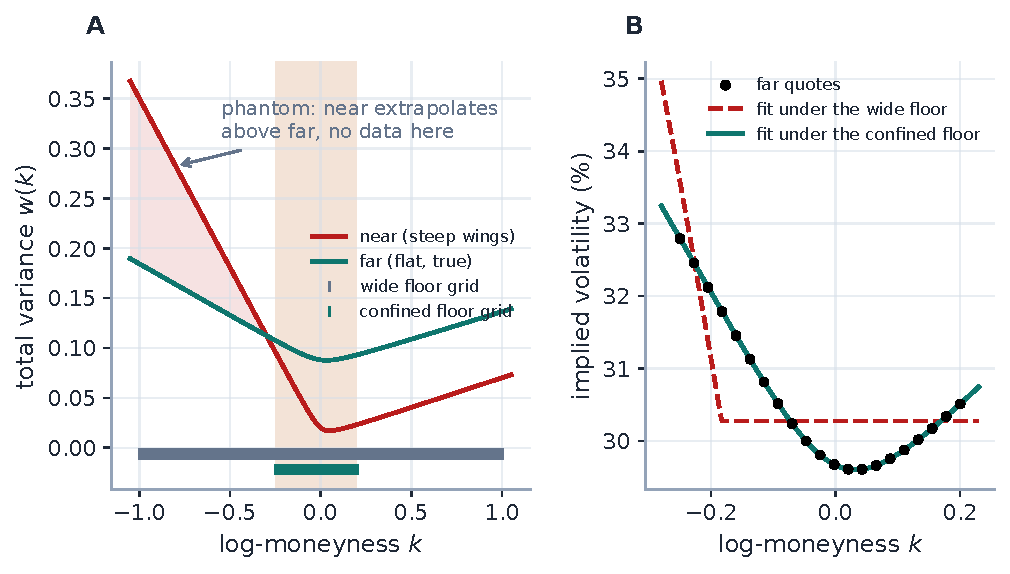
\includegraphics[width=\textwidth]{fig_calm_phantom.pdf}
\caption{The phantom calendar, reproduced with the production
calibrator.  A: on the traded range (shaded) the far slice dominates
--- no true violation --- but the steep near wing extrapolates above
the flat far wing exactly where the wide floor grid (upper ticks)
samples; the confined grid (lower ticks) never looks there.  B: fitted
under the wide-grid floor the far smile flattens away from its own
quotes (\calmphantomwidebp\ vol bp); confined, it is indistinguishable
from the unconstrained fit (\calmphantomdatabp\ vol bp).}
\label{fig:phantom}
\end{figure}

\begin{lstlisting}[caption={The confinement fix (verified against
production to \calmrefagree, \cref{app:ref}).},label={lst:confine}]
def variance_floor_grid_from(k_quotes, n=41):
    k = np.asarray(k_quotes, float)     # floor on the TRADED span only
    if k.size == 0:
        return variance_floor_grid()    # no data at all: wide fallback
    return np.linspace(float(k.min()), float(k.max()), n)
\end{lstlisting}

\subsection{The coordinate matters: why the floor lives in price space}
\label{sec:coordinate}

Confinement has a subtlety the original incident did not expose: for
the LQD face-(iii) constraint, \emph{windowing is not confining}.  The
reason is a two-line locality computation.  Perturb the near slice's
quantile by $\delta Q$ supported on deep-tail levels $u>\alpha_0$
(strikes far beyond any quote).  Then
\[
\delta G(\alpha)=\int_{\max(\alpha,\alpha_0)}^{1}
e^{Q(u)}\,\delta Q(u)\,\dd u
\ \ne0\quad\text{for \emph{every} }\alpha\le\alpha_0 :
\]
$G$ integrates the whole upper tail, so a disagreement between two
extrapolated tails contaminates the comparison at every level below it
--- including levels whose strikes sit squarely inside the quoted
range.  A windowed $G$-floor still reads tail fiction.  The normalized
call at fixed strike has no such reach: $\delta C(k)$ responds only to
density moved across the strike $e^{k}$, so a price-space comparison at
quoted strikes is genuinely local to them.

\Cref{fig:drag} measures exactly this, on the acute scenario of the
shipped confinement lock: a two-day event straddle quoted on a
$\pm6\%$ span under an ordinary three-month slice --- comfortably
ordered on their common support, wildly disagreeing in extrapolation.
Fit the far slice free: \calmdragfreebp\ vol bp of quote error.  Add
the full-grid $G$-floor: \calmdragfullbp\ bp --- the phantom drag.
\emph{Window} the $G$-floor to the common support: still
\calmdragwinbp\ bp, an order of magnitude above clean --- the tail
contamination just derived.  Replace it with the production floor ---
normalized-call ordering $C_{T_2}(k)\ge C_{T_1}(k)$ on the common
support, $\cos^{2}$-tapered at its edges --- and the fit returns to
\calmdragpricebp\ bp, indistinguishable from no floor.  The confined
calendar floor lives in price space because price space is the
coordinate in which ``where'' means anything.

\begin{figure}[H]
\centering
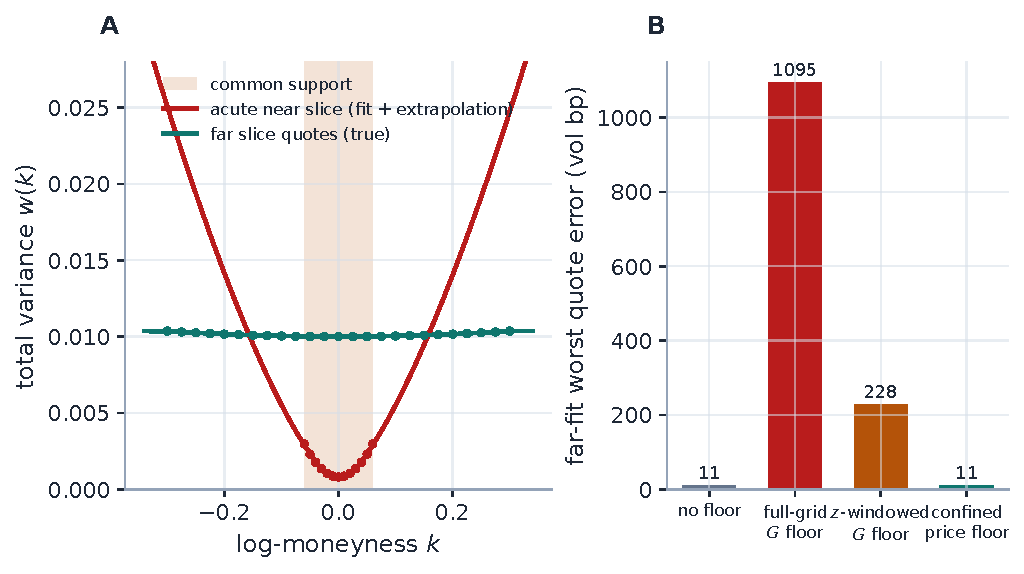
\includegraphics[width=\textwidth]{fig_calm_drag.pdf}
\caption{Windowing is not confining (production fits; the shipped
confinement-lock scenario).  A: an acute two-day slice (rust) quoted
only on the shaded common support, under an ordinary three-month slice
(teal): ordered where both are quoted, disagreeing violently in
extrapolation.  B: the far fit's worst quote error under four floors.
The full-grid $G$-floor drags it \calmdragfullbp\ vol bp off its own
quotes; \emph{windowing} the $G$-floor still leaves \calmdragwinbp\ bp,
because $G(\alpha)$ integrates the entire upper tail
(\cref{sec:coordinate}); the confined price-space floor is
indistinguishable from no floor at \calmdragpricebp\ bp.}
\label{fig:drag}
\end{figure}

\paragraph{Exercise 3.}
The taper margin is $\mathrm{clamp}(0.15\,|W|,\,0.05,\,0.25)$ in
log-moneyness, $|W|$ the common-support width.  For the live surface of
\cref{fig:hero}, the two shortest expiries share a traded span of about
$[-0.04,0.02]$.  Compute the margin, observe that it is nearly as wide
as the window itself, and explain why that is the \emph{intended}
behaviour for 0DTE pairs: with almost no jointly-quoted territory, the
comparison should fade to advisory rather than assert itself on six
strikes.

%======================================================================
\section{Who pays: the symmetric repair}
\label{sec:who}

Everything so far decided \emph{what} to check and \emph{where}.  One
question remains, and it is the note's second original contribution:
when two slices' quotes genuinely conflict --- an event-inverted term
structure, a stale board --- \emph{someone} must concede.  Who?

The historical sequential pass had an implicit answer: expiries are
fitted nearest-to-farthest, each under a floor built from the
already-committed previous slice, so the \emph{latecomer} pays ---
whatever the merits.  On the worked pair of \cref{fig:solver} (a
high-vol $T_1=0.25$ over a calmer $T_2=0.50$, free-fit violation
\calmviolfree\ in total variance) the sequential answer is stark: the
near slice keeps its quotes to \calmseqnearbp\ vol bp while the far
slice is bulldozed \calmseqfarbp\ bp above its own board.  Nothing
about the data justifies that asymmetry --- the near quotes are exactly
as implicated in the inconsistency as the far ones.

The shipped symmetric solver (the production default) replaces the
convention with a declared objective.  Its design is five steps:
\emph{fit independently} (every expiry, warm-seeded, no coupling);
\emph{screen} each adjacent interface with a vega-normalized
call-ordering violation ($0.5$ vol bp tolerance) on the tapered
common-support grid of \cref{sec:coordinate}; \emph{group} violations
into connected components; \emph{jointly refit} each violating
component --- and only it --- by Gauss--Newton on the stacked per-slice
residuals plus tapered interface hinge rows, escalating the interface
weight ($\times10$, at most three times) if a violation survives; and
\emph{fast-path} everything else: a clean ladder's fits are returned
untouched, byte-for-byte --- invariant~3 as an implementation fact,
verified live on SPY (a monotone-PAVA pre-pass was considered and
deliberately dropped: the component joint solve \emph{is} the global
reconciliation, and a second mechanism would fight it).

\begin{figure}[H]
\centering
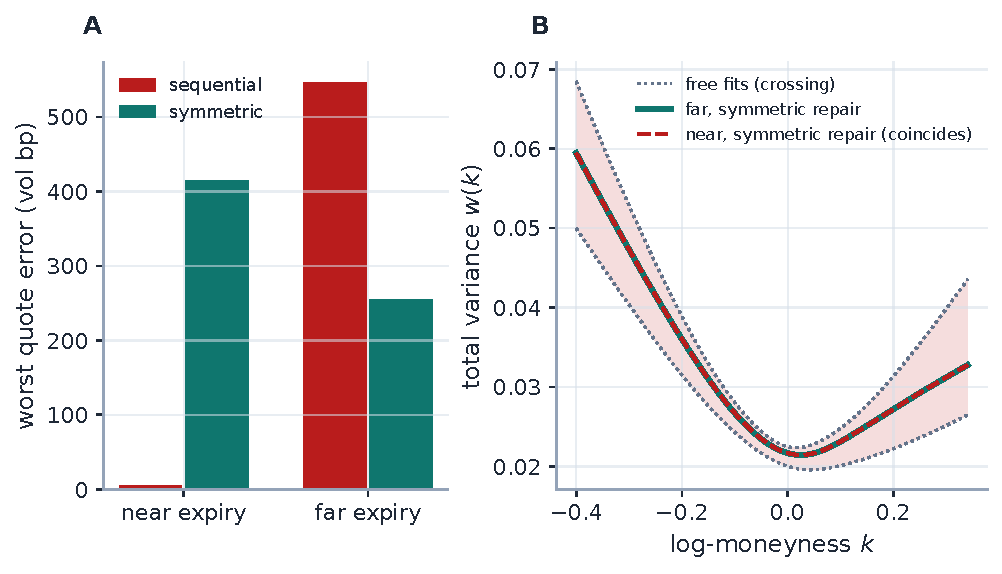
\includegraphics[width=\textwidth]{fig_calm_solver.pdf}
\caption{Who pays, measured (production solvers, identical quotes; an
event-inverted pair with free-fit violation \calmviolfree).  A: the
sequential pass bulldozes the latecomer --- near untouched at
\calmseqnearbp\ vol bp, far conceding \calmseqfarbp\ --- while the
symmetric solver shares the concession
(\calmsymnearbp/\calmsymfarbp\ bp) and lowers the worst-case slice
error.  B: the symmetric repair in variance space: the free fits cross
(shaded); the repaired pair meets on a common curve through the
conflicted region --- the surface is pushed exactly to the boundary of
admissibility, zero forward variance, and no further --- curing the
order to \calmviolcured.}
\label{fig:solver}
\end{figure}

Panel B shows what ``sharing'' converges to: through the conflicted
strikes the repaired near and far slices coincide.  That is not a
solver artefact but the geometry of the constraint set --- the closest
admissible surface to an inverted pair sits on the boundary
$\tvar_{T_1}=\tvar_{T_2}$, i.e.\ exactly zero forward variance, and the
joint least-squares splits the distance to it according to the quote
weights rather than the accident of fitting order.  Under the
extrapolated-region toggle the same joint solve also carries a
\emph{tail contract} per interface --- two seam price rows just beyond
the span union and two wing-slope-order rows (scalar conditions on the
endpoint tails, never pointwise differences of extrapolations: the
phantom lesson, kept by construction).

%======================================================================
\section{The extrapolated region: measure, lean, repair}
\label{sec:extrap}

Confinement enforces \emph{nothing} outside the traded span, and the
region just past the last quote is not worthless --- options there
still carry premium, and a calendar inversion between two \emph{stated}
wing contracts (Note~09) is a real inconsistency even if no quote
witnesses it.  What that region deserves is an explicitly flagged open
problem (2026-07), and production currently answers it in three
graduated phases.  \emph{Measure} (always on): the quality report
computes, over the \emph{time-value envelope} --- strikes beyond the
traded span where the model's own OTM value still exceeds a basis point
of forward --- the worst Durrleman $g$, the worst calendar crossing
against the previous displayed slice, and the wing-slope order; all
advisory, never gating readiness.  \emph{Lean} (opt-in, off by
default): the overlay fits gain three residual blocks over the same
envelope --- a one-curve butterfly hinge, a tapered calendar hinge, and
the scalar wing-slope-order condition --- each budgeted in vol units at
a quarter of an average quote's weight, so the block leans like a
handful of extra quotes and can never outvote the board; on a clean
pair it is a no-op to fit precision, and a genuine mild crossing
($\sim$450 bp) is halved for $\sim$29 bp of traded-range RMS.
\emph{Repair at the boundary} (export only): published curve samples
are lifted, wing by wing outward from the pinned traded edge, onto the
discrete arbitrage-free cone in OTM-price space --- non-increasing,
convex, at or above the previous \emph{published} expiry --- expiries
in ascending maturity; the repair only ever raises wing prices, a clean
wing exports byte-identically, fits and in-app views are untouched, and
a floor exceeding the pinned traded edge (a \emph{core} calendar
conflict, the fit's business, not the exporter's) is capped and flagged
rather than silently repaired.  A repair moves prices, so its
\emph{authority} is confined to the wings even though the constraints
it restores extend there --- Note~09's refinement, applied.

%======================================================================
\section{What is genuinely original here}
\label{sec:original}

The convex-order theory is classical; the contributions are three
pieces of engineering shaped by it.
\begin{enumerate}[leftmargin=1.6em]
\item \emph{One face per model}: recognizing that the LQD asset share
\emph{is} the integrated-quantile curve (\cref{prop:GisA}) makes the
surface diagnostic a free array comparison; the overlays get face (iv)
against whatever the previous display drew; LV needs nothing.  The
same order, checked in each model's own coordinate --- at essentially
zero cost everywhere.
\item \emph{The coordinate half of confinement}
(\cref{sec:coordinate}): the measured demonstration that windowing the
quantile-space floor does not confine it (\calmdragwinbp\ vs
\calmdragpricebp\ vol bp), with the two-line locality computation that
explains why --- and the shipped price-space, cos$^{2}$-tapered,
intersection-support floor it justified.
\item \emph{A declared answer to ``who pays''} (\cref{sec:who}): the
symmetric screen-and-repair solver --- independent fits, local
violation components, one joint Gauss--Newton --- replacing the
sequential pass's blame-the-latecomer convention with the least-squares
split, while keeping clean ladders byte-identical to independent fits
through a verified fast path.
\end{enumerate}

%======================================================================
\section{Limitations}
\label{sec:limits}

Where the guarantees stop.  \emph{The hinge is soft by design}: at
weight $10^{6}$ quotes win a genuine conflict only through the joint
solve's sharing rule, and a sub-tolerance crossing (under the $0.5$
vol bp screen) is deliberately left standing --- the promise is kept to
tolerance, not to machine precision.  \emph{The sharing rule is
statistical, not economic}: the symmetric split follows quote weights,
not any view about which board is stale; a desk that \emph{knows} the
near board is bad should exclude quotes, not expect the solver to
adjudicate.  \emph{Kellerer is an existence theorem only}: the
martingale is not unique, not constructed, and nothing here selects
dynamics --- pricing path-dependent claims still requires a model
(Note~04, Note~12).  \emph{The assumption box is load-bearing}:
stochastic rates break the equivalence between calendar spreads and
the normalized comparison; discrete cash dividends already break the
cash-strike form.  \emph{LV's structural cleanliness is a continuum
statement} policed by a discrete diagnostic, not a proof about the
scheme.  And \emph{the extrapolated region remains an open problem}
(\cref{sec:extrap}): measured always, leaned on only opt-in, repaired
only at the published boundary.
\appendix
%======================================================================
\section{Hyperparameter atlas}
\label{app:atlas}

The only home for settings names: the body speaks mathematics, this
table speaks configuration.

\begin{longtable}{p{0.28\textwidth}p{0.14\textwidth}p{0.50\textwidth}}
\caption{Calendar-arbitrage hyperparameters.}\label{tab:atlas}\\
\toprule Knob & Default & Role\\ \midrule
\endfirsthead \toprule Knob & Default & Role\\ \midrule \endhead
\multicolumn{3}{l}{\emph{Surfaced}}\\ \midrule
\texttt{enforceCalendar} & \texttt{true} & Master toggle for calendar
coupling (all calibration paths).\\
\texttt{surfaceSolver} & \texttt{symmetric} & \texttt{symmetric}
(screen + joint component repair, \cref{sec:who}) or
\texttt{sequential} (nearest-to-farthest with prev-display floors).\\
\texttt{calendarWeight} $W_{\mathrm{cal}}$ & $10^{6}$ & Soft-hinge
strength.  \emph{Not} the graph edge-trust \texttt{calendarWeight} of
Note~14, which shares the name.\\
\texttt{extrapEnforce} & \texttt{false} & Phase-2 tapered
extrapolated-region hinges; under the symmetric solver also arms the
per-interface tail contract (\cref{sec:who}).\\
\midrule
\multicolumn{3}{l}{\emph{Hidden}}\\ \midrule
\texttt{CAL\_STRIDE} & $25$ & LQD full-grid constraint subgrid stride
($\sim$320 points on the $8001$-node grid).\\
\texttt{CAL\_PRICE\_N} & $49$ & Nodes of the confined price-space
floor.\\
\texttt{TAPER\_FRAC/MIN/MAX} & $0.15/0.05/0.25$ & $\cos^{2}$ taper
margin as a clamped fraction of the common-support width
(Exercise~3).\\
\texttt{SCREEN\_TOL\_VOL} & $5\times10^{-5}$ & Symmetric screen
tolerance ($0.5$ vol bp, vega-normalized).\\
\texttt{IFACE\_N} & $33$ & Interface hinge nodes per adjacent pair.\\
\texttt{ESCALATION\_FACTOR} / max & $10$ / $3$ & Interface-weight
escalation when a violation survives a joint pass.\\
\texttt{SEAM\_PAD} & $0.10$ & Tail-contract seam offset beyond the span
union.\\
\texttt{VAR\_FLOOR\_N\_DATA} & $41$ & Confined overlay floor-grid
resolution (\cref{lst:confine}); wide fallback $161$ points on
$[-1,1]$, empty-quotes only.\\
\bottomrule
\end{longtable}

%======================================================================
\section{Performance notes}
\label{app:perf}

\begin{enumerate}[leftmargin=1.6em]
\item The LQD full-grid diagnostic is an array subtraction on the
already-built asset share --- free; its fit-time Jacobian rows are
$-\partial A/\partial\theta$ on active constraints, supplied by
Note~01's analytic Jacobian.
\item The overlay floor is $41$ evaluations of the previous slice's
$\tvar(k)$; the confined price floor is $49$ call evaluations with
taper weights.  Confinement \emph{reduces} work by never sampling the
extrapolation region.
\item The symmetric solver's screen is a handful of vega-normalized
call comparisons per interface; the joint Gauss--Newton runs only over
violation-connected components (block-bidiagonal stacked Jacobian,
analytic, locked against finite differences), so a clean ladder costs
exactly its independent fits plus the screen --- and returns them
byte-for-byte (the fast path; live SPY validation measured
$|\mathrm{sym}-\mathrm{seq}|=0.0$ bp on a clean ladder).
\item All fresh numbers in this edition are produced by the generator
running production calibrators; the live NVDA/SPY incident and the
Phase-2 lean/cost trade ($\sim$450 bp halved at $\sim$29 bp) are
historical, quoted from the test-locked scenarios that reproduce them.
\end{enumerate}

%======================================================================
\section{Traceability}
\label{app:trace}

\begingroup
\small
\setlength{\tabcolsep}{4pt}
\renewcommand{\arraystretch}{1.15}
\begin{longtable}{@{}p{0.42\textwidth}p{0.10\textwidth}p{0.44\textwidth}@{}}
\caption{Claims in this note and the code/tests that lock them.}
\label{tab:trace}\\
\toprule Claim & Object & Code anchor \newline \emph{Test anchor}\\ \midrule
\endfirsthead
\toprule Claim & Object & Code anchor \newline \emph{Test anchor}\\ \midrule
\endhead
LQD integrated-quantile constraint; surface repair &
\cref{prop:GisA}, \eqref{eq:slack} &
\nolinkurl{volfit/calib/calendar.py},
\nolinkurl{volfit/models/lqd/calibrate.py}\newline
\nolinkurl{tests/test_surface.py::test_violating_quotes_get_repaired_when_enforced}\\
\addlinespace
Overlay floor reads the previous slice's $\tvar$; crushes real
violations (SVI, MCS) &
\eqref{eq:wfloor} &
\nolinkurl{volfit/calib/calendar.py}\newline
\nolinkurl{tests/test_overlay_calendar.py::test_variance_floor_reads_prev_total_variance};
\nolinkurl{::test_svi_floor_crushes_calendar_violation};
\nolinkurl{::test_sigmoid_floor_crushes_calendar_violation}\\
\addlinespace
Byte-identical with no floor / toggle off &
invariant~3 &
\nolinkurl{volfit/models/svi_jw/calibrate.py},
\nolinkurl{volfit/models/sigmoid/calibrate.py}\newline
\nolinkurl{tests/test_overlay_calendar.py::test_svi_no_floor_is_byte_identical};
\nolinkurl{::test_build_display_fit_no_floor_byte_identical}\\
\addlinespace
Phantom scenario: consistent on data, phantom in wings; confined grid
fits clean, wide grid flattens &
\cref{fig:phantom} &
\nolinkurl{volfit/calib/calendar.py}\newline
\nolinkurl{tests/test_overlay_calendar.py::test_far_above_near_inside_data_but_not_in_wings};
\nolinkurl{::test_wide_grid_breaks_svi_but_data_grid_does_not}\\
\addlinespace
Price-space confinement kills the drag; support/taper geometry &
\cref{fig:drag} &
\nolinkurl{volfit/calib/calendar.py}\newline
\nolinkurl{tests/test_calendar_confinement.py::test_confined_floor_kills_the_phantom_calendar_drag};
\nolinkurl{::test_common_support_intersection_and_disjoint};
\nolinkurl{::test_support_taper_shape};
\nolinkurl{::test_confined_floor_is_the_near_call_curve_on_common_support}\\
\addlinespace
Symmetric solver: fast path; local components; symmetric split;
analytic stacked Jacobian; tail contract &
\cref{sec:who} &
\nolinkurl{volfit/calib/symmetric.py},
\nolinkurl{symmetric_stack.py}\newline
\nolinkurl{tests/test_symmetric_surface.py::test_clean_ladder_is_exactly_the_independent_fits};
\nolinkurl{::test_repair_is_local_to_the_violation_component};
\nolinkurl{::test_real_violation_is_shared_symmetrically};
\nolinkurl{::test_stacked_jacobian_matches_finite_differences};
\nolinkurl{::test_tail_contract_orders_the_extrapolated_wings};
\nolinkurl{::test_acute_phantom_ladder_does_not_trigger_the_solver}\\
\addlinespace
prev\_display threaded ascending-$T$ everywhere (sequential path) &
\cref{sec:cheap} &
\nolinkurl{volfit/api/service.py},
\nolinkurl{volfit/api/workflow.py}\newline
\nolinkurl{tests/test_calibration_workflow.py::test_enforce_calendar_threads_prev_into_parametric_items};
\nolinkurl{::test_enforce_calendar_threads_prev_overlay_for_non_lqd}\\
\addlinespace
Coupled surface arbitrage-free; certification &
\cref{thm:faces} &
\nolinkurl{volfit/api/workflow.py},
\nolinkurl{backend/backtest/certification.py}\newline
\nolinkurl{tests/test_calibration_workflow.py::test_enforce_calendar_surface_is_arbitrage_free};
certification case \texttt{symmetric\_calendar}\\
\bottomrule
\end{longtable}
\endgroup

%======================================================================
\section{Reference implementation}
\label{app:ref}

The enforcement residuals are one line each; the confined grid is
\cref{lst:confine}, verified against production output to
\calmrefagree\ on quoted and empty inputs alike.  The hinges below
reproduce the residual blocks inside the calibrators exactly (the
production rows are inline in each calibrator --- deliberately, since
each model evaluates its own face of \eqref{eq:faces}):

\begin{lstlisting}[caption={The calendar hinges as they appear (inline)
in the calibrators: face (iv) for the overlays, face (iii) on the LQD
grid, face (i) with taper for the confined price floor and the
symmetric interfaces.}]
# SVI / MCS (face (iv)): rows are zero unless the far dips
cal = np.sqrt(calendar_weight) * np.maximum(cal_floor - w_model, 0.0)

# LQD full grid (face (iii)): the same hinge on the asset share A(z)
cal = np.sqrt(cal_weight) * np.maximum(cal_floor - slice_.asset_share_at(cal_z), 0.0)

# Confined price floor / symmetric interface (face (i)), cos^2-tapered
calk = np.sqrt(cal_weight) * taper * np.maximum(price_floor - slice_.call_price(cal_k), 0.0)
\end{lstlisting}

\begin{thebibliography}{9}
\bibitem{Strassen1965} V.~Strassen.  The existence of probability
measures with given marginals.  \emph{Ann.\ Math.\ Statist.},
36(2):423--439, 1965.
\bibitem{Kellerer1972} H.~Kellerer.  Markov-Komposition und eine
Anwendung auf Martingale.  \emph{Math.\ Ann.}, 198:99--122, 1972.
\bibitem{HPRY2011} F.~Hirsch, C.~Profeta, B.~Roynette and M.~Yor.
\emph{Peacocks and Associated Martingales}.  Springer, 2011.
\bibitem{CarrMadan2005} P.~Carr and D.~Madan.  A note on sufficient
conditions for no arbitrage.  \emph{Finance Research Letters},
2(3):125--130, 2005.
\bibitem{GatheralJacquier2014} J.~Gatheral and A.~Jacquier.
Arbitrage-free SVI volatility surfaces.  \emph{Quantitative Finance},
14(1):59--71, 2014.
\end{thebibliography}

\end{document}
